\documentclass{standalone}
\usepackage{tikz}
\usepackage{pgfplots}
\pgfplotsset{compat=1.18}
\usepackage{amsmath}
\begin{document}

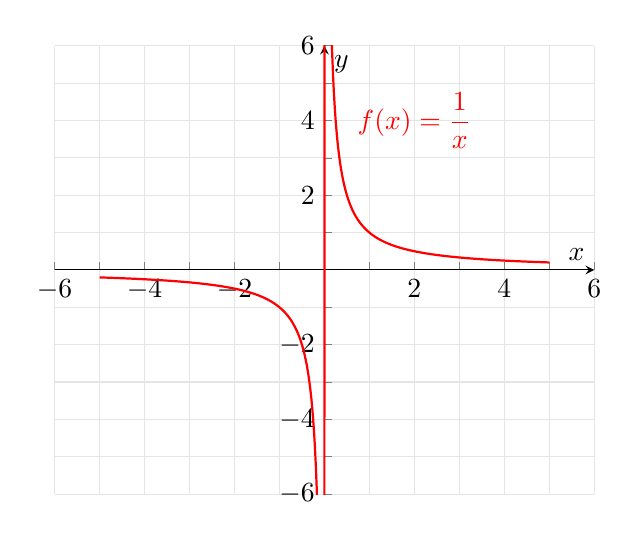
\begin{tikzpicture}
	\fontsize{10}{12}\selectfont
    \def\MAX{6} % 定义 MAX 变量,值为 6
    \begin{axis}[
        axis lines = middle,
        xlabel = {$x$},
        ylabel = {$y$},
        xmin = -\MAX, xmax = \MAX,
        ymin = -\MAX, ymax = \MAX,
        grid = both,
        minor tick num = 1,
        major tick length = 0.1cm,
        grid style = {black!10},
        xtick = {-6, -4, -2, 0, 2, 4, 6},
        ytick = {-6, -4, -2, 0, 2, 4, 6},
        domain = -\MAX:\MAX,
        xtick align=inside, % 将主刻度线对齐到坐标轴内侧
        ytick align=inside,  % 将主刻度线对齐到坐标轴内侧
    ]
    % 绘制函数y=1/x
    \addplot[red, domain=-\MAX+1:\MAX-1, samples=500, thick] {(1/x)};

    \node at (2,4) [red] {$f(x)=\dfrac{1}{x}$}; 
    \end{axis}
\end{tikzpicture}

\end{document}